\documentclass[a4paper, 11pt]{article}

\usepackage[utf8]{inputenc}
\usepackage[slovak]{babel}
\usepackage[T1]{fontenc}
\usepackage[margin=2.5cm]{geometry}
\usepackage{graphicx}
\usepackage{hyperref}
\usepackage{xcolor}
\usepackage{enumitem}
\usepackage{parskip}
\usepackage[htt]{hyphenat}

% Povoliť zalamovanie v \texttt{} fontoch (rieši overfull hbox pri dlhých
% identifikátoroch ako InterpreterError(INT_DNU))
\sloppy

\hypersetup{
    colorlinks=true,
    linkcolor=black,
    urlcolor=blue
}

\title{IPP 2025/2026 -- Projekt: Interpret jazyka SOL26 \\
\large Dokumentácia vylepšenej verzie}
\author{Ľuboš Noska (xnoskal00) \\ FIT VUT v Brne}
\date{\today}

\begin{document}

\maketitle

\section{Celkový popis návrhu riešenia}

Jadrom môjho riešenia je trieda \texttt{Evaluator} spolu s runtime triedami
\texttt{SOLClass}, \texttt{SOLObject} a \texttt{Environment}. Tieto triedy
nesú celú logiku behu programu -- od vytvárania inštancií cez posielanie
správ až po vyhľadávanie metód v~reťazci dedičnosti. Trieda \texttt{Interpreter}
(ktorej kostra bola súčasťou šablóny) nad nimi zastrešuje životný cyklus
programu: registráciu užívateľských tried zo vstupu, statickú kontrolu arity
metód a spustenie metódy \texttt{run} triedy \texttt{Main}.

Runtime model som navrhol minimalisticky. Každá hodnota v~programe je
\texttt{SOLObject}, každá trieda je \texttt{SOLClass} a každé volanie metódy
alebo bloku vytvorí nové \texttt{Environment}. Pydantic uzly z~AST som
neprekladal do žiadnej druhej medzireprezentácie -- \texttt{Evaluator} ich
vyhodnocuje priamo. Vďaka tomu mám celý strom kedykoľvek k~dispozícii
(napríklad pri closure prostrediach blokov) a vyhol som sa duplicite
dvoch paralelných reprezentácií programu.

Posielanie správ je implementované jednou univerzálnou metódou
\texttt{\_eval\_send}, ktorá postupne skúša tri cesty: (1) vyhľadanie
užívateľskej metódy v~reťazci dedičnosti, (2) vstavanú metódu podľa
najbližšieho vstavaného predka a (3) prácu s~inštančnými atribútmi
(getter alebo setter podľa selektora a počtu argumentov). Ak ani jedna cesta
neuspeje, vyhodí sa chyba~51. Dispatcher pre vstavané triedy
(\texttt{\_dispatch\_builtin}) deleguje podľa typu na špecializované metódy
(\texttt{\_dispatch\_string}, \texttt{\_dispatch\_integer},
\texttt{\_dispatch\_bool}, \texttt{\_dispatch\_nil},
\texttt{\_dispatch\_block}) s~fallbackom na \texttt{\_dispatch\_object}.
Toto rozdelenie podľa typu som zvolil, aby bol každý dispatcher krátky
a aby pridanie novej vstavanej metódy nevyžadovalo zásah do hlavnej
dispatch logiky.

Najviac času som strávil nad rozlíšením \texttt{self}, \texttt{super}
a bežnej referencie pri dedičnosti metód. V~\texttt{Environment} si preto
držím atribút \texttt{current\_class}, ktorý označuje triedu, v~ktorej je
aktuálne bežiaca metóda \emph{definovaná} (nie triedu objektu).
\texttt{super} potom začína vyhľadávanie od rodiča tejto triedy, nie od
triedy prijímateľa -- inak by neprechádzali testy s~viacúrovňovou
dedičnosťou.

\textbf{UML diagram tried} je uvedený na obrázku~\ref{fig:uml}. Triedy
prevzaté zo šablóny sú odlíšené \emph{šedou} farbou, trieda \texttt{Interpreter}
(ktorej kostra bola súčasťou šablóny, ale hlavná logika je moja) je
\emph{svetložltá} a moje vlastné runtime triedy a modul vstavaných tried sú
\emph{svetlomodré}.

\begin{figure}[h!]
    \centering
    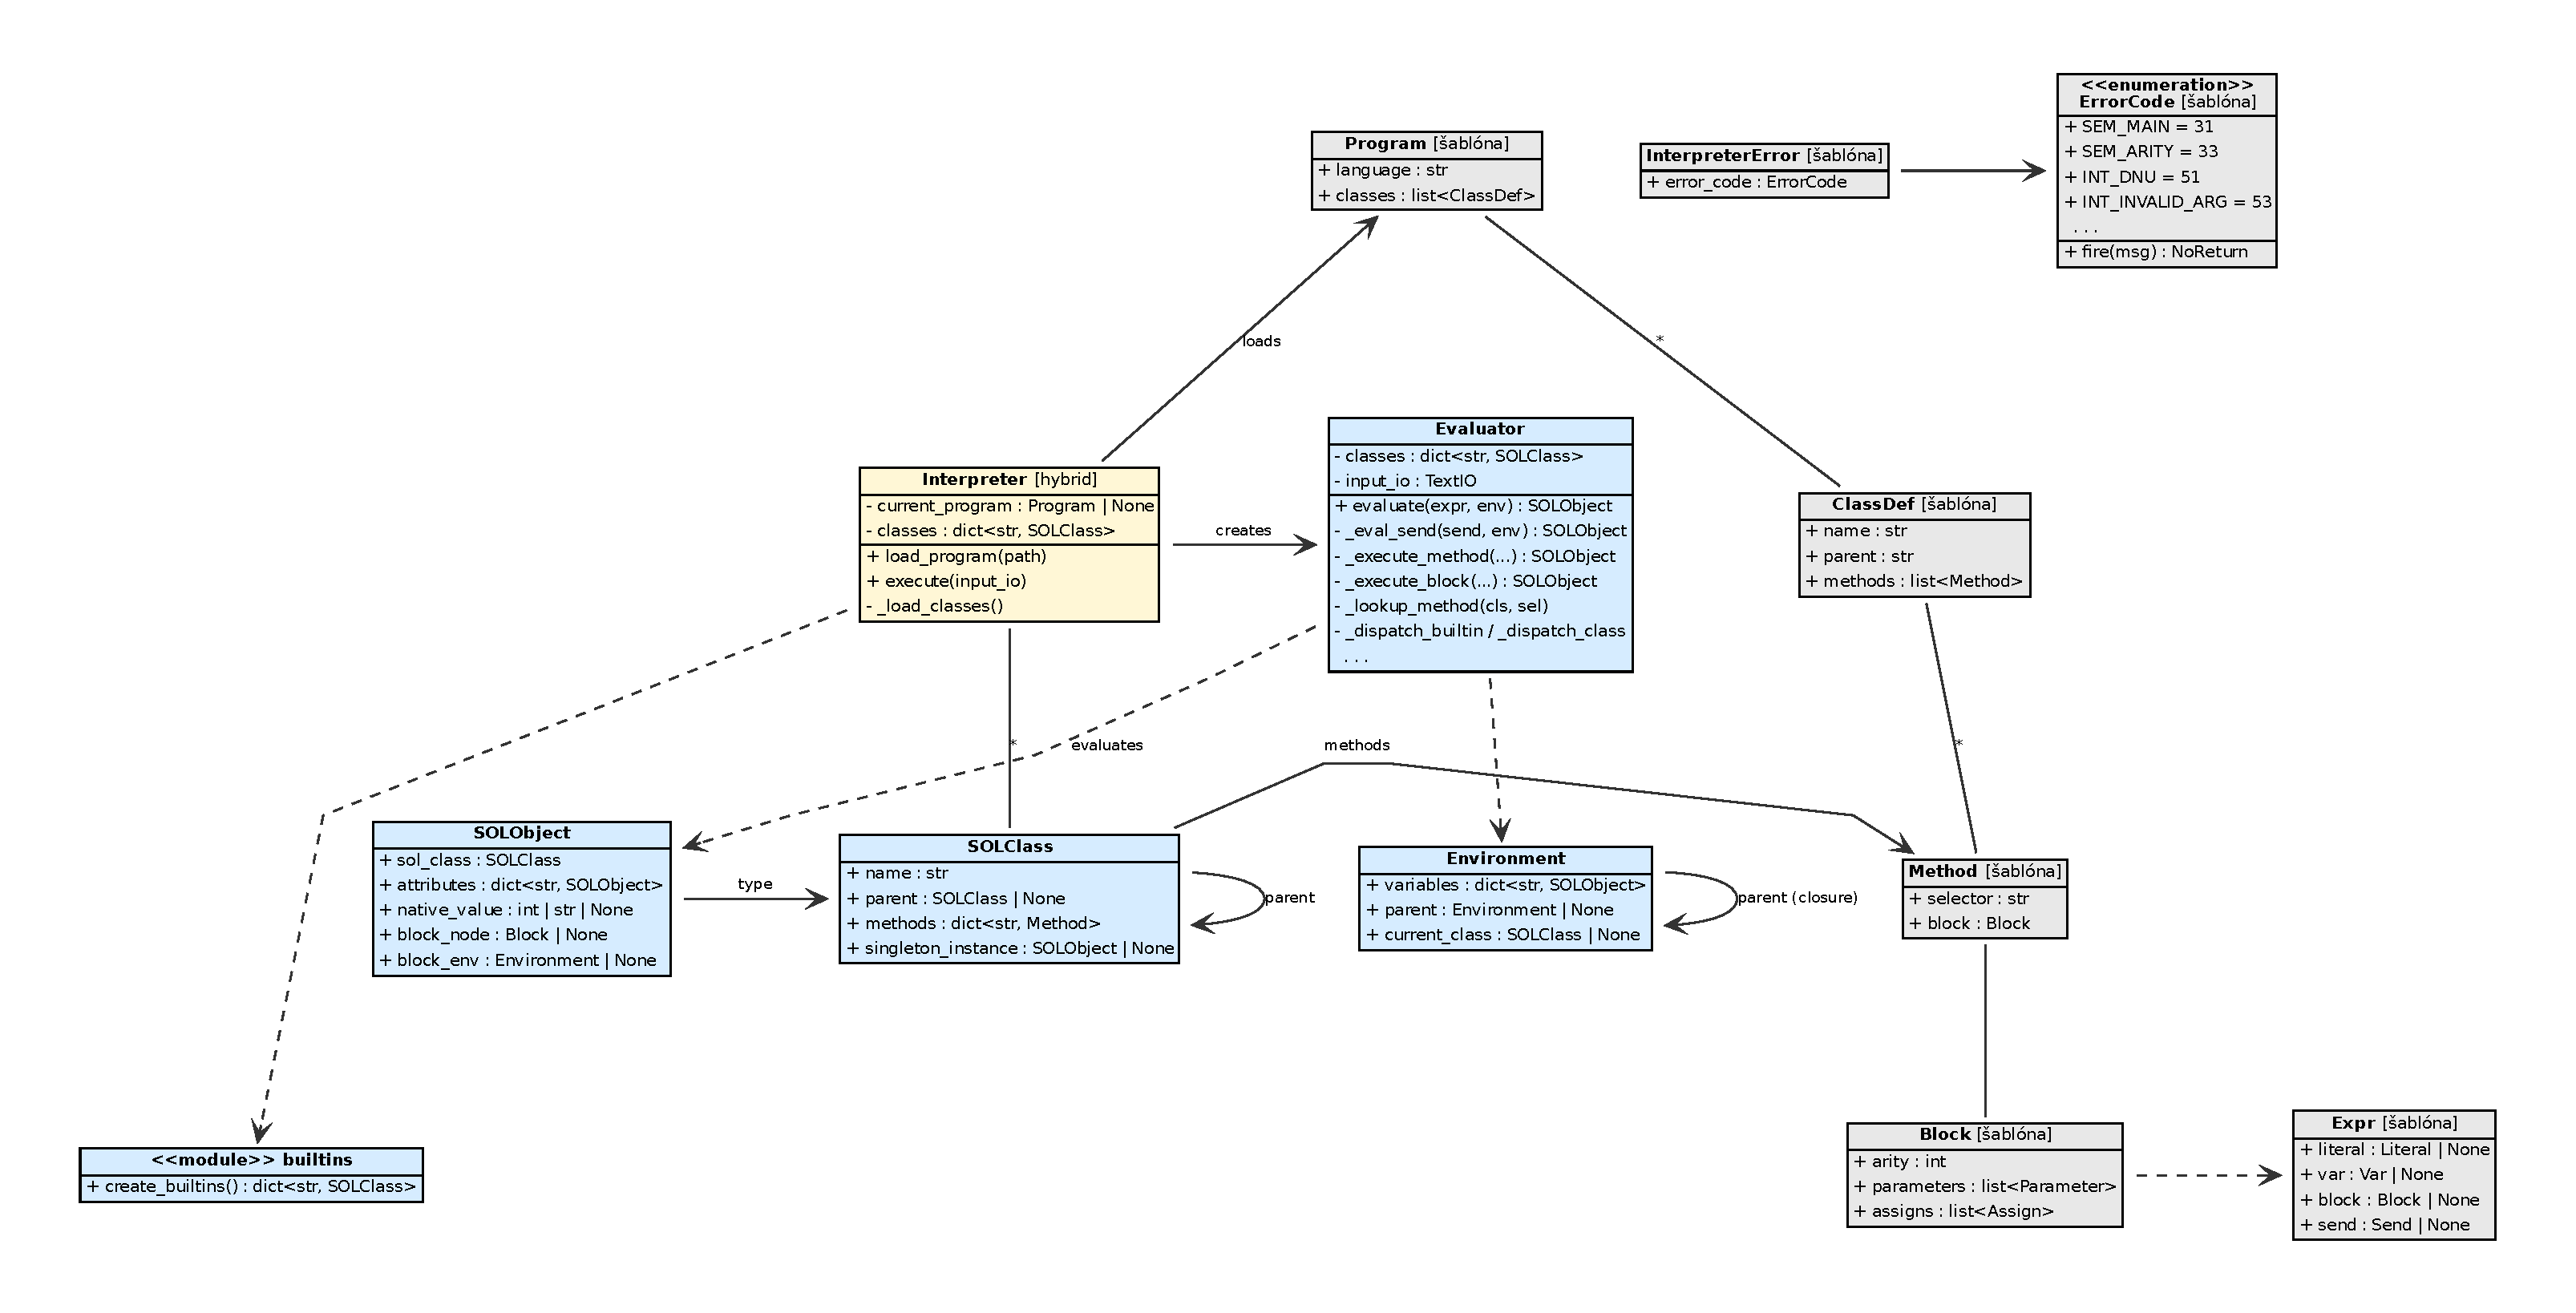
\includegraphics[width=\textwidth]{uml.pdf}
    \caption{UML diagram tried interpretu SOL26. Šablónové triedy sú šedé,
    hybridná trieda \texttt{Interpreter} je žltá, moje triedy sú modré.}
    \label{fig:uml}
\end{figure}

\section{Popis hlavných interných dátových štruktúr}

\textbf{\texttt{SOLClass}} reprezentuje triedu počas behu programu. Obsahuje
meno, odkaz na rodiča (\texttt{parent}), slovník metód (selektor~$\to$
pydantic uzol \texttt{Method}) a voliteľne \texttt{singleton\_instance} pre
triedy \texttt{Nil}, \texttt{True} a \texttt{False}, u~ktorých musí
\texttt{new}/\texttt{from:} vždy vrátiť tú istú inštanciu.

\textbf{\texttt{SOLObject}} je jediná trieda pre každý objekt v~behu
programu -- pre užívateľské inštancie, vstavané čísla, reťazce, booleany, \texttt{nil}
aj bloky. Okrem odkazu na svoju triedu a slovníka \texttt{attributes} drží
\texttt{native\_value} (natívna Python hodnota pre \texttt{Integer}
a~\texttt{String}), dvojicu \texttt{block\_node} a \texttt{block\_env}
(keď je objekt blokom -- telo a zachytené closure prostredie) a~dvojicu
\texttt{is\_class\_ref} a~\texttt{referred\_class} (keď je objekt
~,,literálom triedy`` ako \texttt{Integer}, ktorému možno poslať \texttt{new}).

\textbf{\texttt{Environment}} je premenné prostredie jedného volania metódy
alebo bloku. Drží slovník lokálnych premenných, odkaz na rodičovský scope
(pre closures blokov) a aktuálnu definičnú triedu metódy. Vyhľadávanie
premennej prechádza \texttt{parent} reťazec až po najvrchnejšie prostredie,
čo automaticky podporuje uzávery.

\textbf{\texttt{Evaluator}} je trieda bez stavu vo vzťahu k~programu --
vlastní len \texttt{classes} (register všetkých tried) a \texttt{input\_io}
(štandardný vstup). Všetky medziľahlé dáta počas behu putujú cez parametre,
čo výrazne uľahčuje uvažovanie o~rekurzii a closure sémantike.

\section{Využitie návrhových vzorov a princípov OOP}

\textbf{Interpreter pattern.} Celé jadro je priamočiara implementácia
návrhového vzoru Interpreter. Uzly AST (\texttt{Expr} a jeho varianty) sú
~,,gramatika`` a trieda \texttt{Evaluator} má jednu metódu \texttt{evaluate},
ktorá rekurzívne vyhodnocuje ľubovoľný uzol. Rozšírenie o nový typ výrazu by
znamenalo pridať novú vetvu do \texttt{evaluate} a novú privátnu metódu
\texttt{\_eval\_<typ>} -- všetko ostatné zostáva nedotknuté.

\textbf{Strategy / dispatch tables.} Vyhodnocovanie správ vstavaných tried
využíva niečo medzi tabuľkou funkcií a stratégiou: \texttt{\_dispatch\_builtin}
podľa najbližšieho vstavaného predka delegovaním zavolá jednu zo špecializovaných
dispatcher metód (\texttt{\_dispatch\_string}, \texttt{\_dispatch\_integer},
\ldots). Tie vrátia \texttt{None}, ak daný selektor nepoznajú -- \texttt{None}
je potom signál, že sa má vyskúšať fallback na \texttt{Object}. Tento prístup
mi dovolil pridávať nové vstavané metódy bez zmeny hlavnej dispatch logiky
a zároveň podporuje dedičnosť od vstavaných tried (užívateľská \texttt{MyInt
: Integer} automaticky ,,dedí`` všetky celočíselné operácie).

\textbf{Composite.} Objekt aj trieda majú spoločný polymorfný záujem na
atribúte \texttt{parent} -- v \texttt{SOLClass} ide o~dedičnosť,
v~\texttt{Environment} o~vnorenie scope. Obidve je možné prechádzať rovnakým
while-cyklom (\texttt{while current is not None: ...; current = current.parent}),
čo robí pomocné metódy \texttt{\_lookup\_method}, \texttt{\_builtin\_base}
a \texttt{\_eval\_var} veľmi krátkymi a podobnými.

\textbf{Encapsulation a princíp jednej zodpovednosti.} Každý súbor má jasnú
úlohu -- \texttt{error\_codes} kódy chýb, \texttt{input\_model} štruktúru
vstupu, \texttt{sol\_object} runtime reprezentáciu, \texttt{builtins}
inicializáciu vstavaných tried, \texttt{interpreter} životný cyklus programu
a \texttt{evaluator} samotné vyhodnotenie. Vďaka tomu sa po každej úprave
jasne dá povedať, ktorého modulu sa zmena týka -- napríklad pri oprave
testov \textsc{inheritance} som menil len \texttt{evaluator} a~pri oprave
\textsc{semerr\_arity} len \texttt{interpreter}.

\textbf{Singleton.} Triedy \texttt{Nil}, \texttt{True} a \texttt{False}
využívajú Singleton -- \texttt{SOLClass} má nepovinný atribút
\texttt{singleton\_instance} a celá logika (\texttt{new}, \texttt{from:},
literál) sa cezeň zjednocuje do jedinej kontroly.

\section{Popis najväčších problémov}

\textbf{Dispatch \texttt{super} v blokoch.} Prvý problém, pri ktorom som
narazil na strop, bolo, že keď je \texttt{super} použitý vo vnorenom bloku
v~metóde, pôvodný návrh (kde \texttt{current\_class} bolo len v~najvrchnejšom
prostredí metódy) nevedel túto informáciu cez hranice blokov preniesť.
Opravil som to metódou \texttt{\_get\_current\_class}, ktorá prechádza
\texttt{parent} reťaz prostredí a vráti najbližšie neprázdne
\texttt{current\_class}. Keďže uzávery bloku odkazujú na prostredie metódy,
informácia sa nikdy nestratí.

\textbf{Dedičnosť od vstavaných tried.} Druhý problém súvisel s užívateľskou
triedou, ktorá dedí priamo alebo nepriamo od \texttt{Integer}, \texttt{String}
a pod. Keď takej inštancii program poslal \texttt{plus:} alebo \texttt{asString},
pôvodný dispatcher to nerozpoznal, lebo sa pozeral len na presné meno
\texttt{sol\_class.name}. Riešením je pomocná metóda \texttt{\_builtin\_base},
ktorá nájde najbližšieho \emph{vstavaného} predka danej triedy. Dispatch potom
funguje rovnako pre \texttt{Integer} aj pre užívateľskú \texttt{PositiveInt
: Integer}.

\textbf{Poradie dispatchu vs. metódy \texttt{Object}.} Nakoniec -- keďže
každá užívateľská trieda implicitne dedí od \texttt{Object}, musel som
rozhodnúť, v akom poradí sa skúšajú užívateľské a vstavané metódy. Správne
poradie je: najprv užívateľské metódy v reťazi dedičnosti, potom vstavané
metódy pre typ (ak sa jedná o vstavaný typ alebo jeho potomka), a nakoniec
vstavané metódy \texttt{Object} (napríklad \texttt{asString},
\texttt{identicalTo:}). Inak by užívateľ nemohol prepísať \texttt{asString}
v~svojej triede.

\section{Rozsah a dôvod úprav vo vylepšenej verzii}

Pôvodné odovzdanie získalo v automatickom hodnotení $3{,}5/7{,}75$~bodu.
Najväčšie straty boli v kategóriách \textsc{semerr\_arity} (0/40),
\textsc{complex} (0/50), \textsc{inheritance} (1/12), \textsc{class} (2/9)
a \textsc{closure} (3/14). Vylepšenia smerujú práve do týchto oblastí.
Nižšie sú všetky zmeny chronologicky.

\subsection*{Interpret}

\begin{itemize}[nosep]
    \item \textbf{Statická kontrola arity selektorov} (kategória
    \textsc{semerr\_arity}). V~\texttt{\_load\_classes} som doplnil
    porovnanie počtu dvojbodiek v~selektore s~počtom parametrov príslušného
    bloku a pri nezhode sa vyhadzuje chyba~33. Predtým sa nezhoda
    detekovala až dynamicky pri volaní, čím zlyhávali všetky testy, ktoré
    očakávali statickú detekciu.
    \item \textbf{Dedičnosť metód} (kategórie \textsc{inheritance},
    \textsc{class}, \textsc{complex}). Metóda \texttt{\_lookup\_method} teraz
    vracia dvojicu (nájdená metóda, trieda kde bola definovaná). Táto
    ,,definičná trieda`` putuje do \texttt{Environment.current\_class},
    vďaka čomu \texttt{super} hľadá v~správnom bode hierarchie aj pri
    viacúrovňovej dedičnosti. Pribudli pomocné
    \texttt{\_get\_current\_class} (získa informáciu cez \texttt{parent}
    reťaz prostredí, čím funguje aj z~vnorených blokov)
    a \texttt{\_builtin\_base} (nájde najbližšieho vstavaného predka,
    čo umožňuje dedičnosť od \texttt{Integer}, \texttt{String} a pod.).
    Upravil som aj poradie dispatchu v \texttt{\_eval\_send} -- najprv
    užívateľské metódy v reťazi dedičnosti, až potom vstavané -- aby ich
    bolo možné prepísať.
    \item \textbf{Konštruktor \texttt{from:}} (kategória \textsc{class},
    \textsc{rterr\_arg}). Do \texttt{\_dispatch\_class} pribudla kontrola
    typu argumentu cez \texttt{\_is\_instance\_of}. Ak argument nie je
    inštanciou prijímateľa ani jeho potomka, vyhadzuje sa chyba~53.
    \item \textbf{Singletony \texttt{Nil}/\texttt{True}/\texttt{False}}
    (kategória \textsc{advanced}). Opravil som dispatchery tak, aby
    \texttt{new} a \texttt{from:} na týchto triedach vždy vracali tú istú
    inštanciu uloženú v~\texttt{SOLClass.singleton\_instance}. Zároveň
    som doladil vstavané predikáty \texttt{isNumber}, \texttt{isString},
    \texttt{isBlock}, \texttt{isNil} a \texttt{isBoolean}, ktoré
    nevracali správnu hodnotu pre potomkov vstavaných tried.
    \item \textbf{Triedna metóda \texttt{String read} a \texttt{Block new}.}
    \texttt{read} bol predtým ošetrený len ako inštančná metóda --
    presunul som ho do \texttt{\_dispatch\_class} tak, aby sa dal volať
    ako \texttt{String read}. Podobne \texttt{Block new} teraz vytvára
    korektný prázdny blok s~arity~0, nie obyčajný \texttt{Object}.
\end{itemize}

\subsection*{Kontajnerizácia}

\textbf{Predvolený \texttt{--interpreter} v~test stage.} Pôvodne sa
tester spúšťal bez argumentov, čo od používateľa vyžadovalo, aby
vždy odovzdal \texttt{--interpreter}. Nový \texttt{ENTRYPOINT} má
tento argument prednastavený na \texttt{python3 /src/int/src/solint.py},
takže priamo ukazuje na interpret v~rovnakom obraze. Užívateľ ho môže
kedykoľvek prepísať vlastným \texttt{--interpreter}, keďže ďalšie CLI
argumenty sa štandardne pridávajú za hodnoty z~\texttt{ENTRYPOINT}.

\textbf{Wrappery pre nástroje kvality kódu.} Aktualizovaný skript
\texttt{is\_archive\_ok.sh} testuje dostupnosť nástrojov kvality
(\texttt{ruff}, \texttt{mypy}, \texttt{eslint}, \texttt{prettier})
tak, že nad \texttt{/src/int/} a \texttt{/src/tester/} v~kontajneri
namontuje obsah archívu. Pôvodné riešenie vytváralo symlinky na tieto
nástroje až počas \texttt{docker build} -- mount ich potom prekryl
a~nástroje prestali byť viditeľné. Preto som do \texttt{int/}
a~\texttt{tester/} pridal malé shell wrappery \texttt{ruff}, \texttt{mypy},
\texttt{eslint}, \texttt{prettier}, ktoré sú súčasťou archívu
a~prežijú mount. V~\texttt{check} stage som navyše pridal
\texttt{npm install -g eslint prettier}, aby boli globálne dostupné
bez ohľadu na to, či je \texttt{/src/tester/node\_modules/}
po~mount-e dostupný. Samotný build-time lint som prepol na priame
volanie \texttt{./node\_modules/.bin/eslint} a~\texttt{./node\_modules/.bin/prettier},
aby používal verzie zamknuté v~\texttt{package-lock.json}.

\subsection*{Testovací nástroj a dokumentácia}

V testovacom nástroji som nerobil funkčné zmeny -- úpravy sa týkali
výlučne interpretu a Dockerfile. Samotná dokumentácia bola
aktualizovaná o~túto sekciu a o~popis nových pomocných metód
(\texttt{\_builtin\_base}, \texttt{\_get\_current\_class},
\texttt{\_is\_instance\_of}) v~sekciách 1 a~4.

\section{Popis využitia prostriedkov AI v projekte}

V projekte som využíval chatbot \textbf{Gemini} (Google) ako
doplnkovú pomôcku pri porozumení zadania a~vlastného kódu.
Konkrétne som ho používal na:

\begin{itemize}[nosep]
    \item \textbf{Vysvetľovanie šablóny projektu} -- na začiatku som si
    dal postupne vysvetliť jednotlivé súbory šablóny (napr.
    \texttt{input\_model.py}, \texttt{solint.py}, \texttt{error\_codes.py}),
    aby som sa rýchlejšie zorientoval v~tom, čo je už pripravené a~kde
    budem dopĺňať vlastnú logiku.
    \item \textbf{Orientáciu v~zadaní a~špecifikácii SOL26} -- pýtal som
    sa na význam jednotlivých sekcií zadania, formát \texttt{.test}
    súborov, pravidlá hodnotenia a~štruktúru SOL-XML. Využil som to
    hlavne vtedy, keď som si nebol istý interpretáciou niektorej pasáže
    špecifikácie.
    \item \textbf{Písanie SOL-XML testovacích súborov} -- nechal som si
    generovať vstupné XML scenáre (napr. \texttt{test\_class*.xml},
    \texttt{test\_closure*.xml}, \texttt{test\_singletons.xml}), na ktorých
    som si priebežne overoval, či interpret funguje správne a~či
    novo implementovaná funkcionalita neporušila skôr prejdené testy.
    \item \textbf{Písanie docstringov} -- pri hotových moduloch som ho
    požiadal o~vygenerovanie docstringov pre triedy a~metódy.
    \item \textbf{Diskusiu nad návrhom} -- napríklad pri rozhodovaní,
    či singletonovú logiku riešiť v~\texttt{SOLClass} alebo
    v~dispatcheri, alebo prečo musí \texttt{\_lookup\_method} vracať aj
    triedu, v~ktorej bola metóda definovaná.
\end{itemize}

Screenshoty z~týchto konverzácií sú priložené v~adresári \texttt{ai/}
v~koreni archívu.

\section{Možnosti ďalšieho rozšírenia}

Zo zoznamu rozšírení som si vybral dve, ktoré by bolo možné zapracovať
s~malým zásahom do existujúceho návrhu.

\subsection*{Podpora mechanizmu \texttt{doesNotUnderstand}}

Aktuálne v~\texttt{\_eval\_send} končia všetky neúspešné dispatch pokusy
chybou~51. Rozšírenie by znamenalo zmeniť len tento jeden bod: namiesto
chyby by sa na príjemcovi skúsilo poslať \texttt{doesNotUnderstand:}
s~argumentom typu \texttt{Message}. \texttt{Message} by bola nová vstavaná
trieda s~atribútmi \texttt{selector} a \texttt{args} a vstavanými metódami
\texttt{selector}, \texttt{argumentAt:} a \texttt{argumentCount}. Registroval
by som ju v~\texttt{create\_builtins} a pridal dispatcher
\texttt{\_dispatch\_message}. Predvolenú implementáciu
\texttt{doesNotUnderstand:} by poskytol \texttt{\_dispatch\_object} --
vyhodil by pôvodnú chybu~51. Proti nekonečnej rekurzii stačí na
\texttt{Evaluator} držať množinu už prebiehajúcich DNU dvojíc
(príjemca, selektor).

\subsection*{Podpora rozhraní (\texttt{interface})}

V~pydantic modeli by pribudla nová trieda \texttt{InterfaceDef} s~atribútmi
\texttt{name}, \texttt{extends} (zoznam nadradených rozhraní) a
\texttt{selectors} (povinné metódy); \texttt{ClassDef} by dostal voliteľný
atribút \texttt{implements}. Novú runtime štruktúru nepotrebujem -- stačí
v~\texttt{Interpreter} viesť druhý register \texttt{interfaces}. Kontrolu
urobím staticky v~\texttt{\_load\_classes}: pre každú triedu s~\texttt{implements}
overím, že každý selektor rozhrania (vrátane zdedených) je nájditeľný cez
existujúce \texttt{\_lookup\_method}, a pri nesplnení vyhodím chybu~35.
Zákaz inštanciácie rozhrania pridám jednou vetvou
v~\texttt{\_dispatch\_class}.

\end{document}
